\section{Introduction}

\frame[<+->]{
	\frametitle{Course details}
	
	\begin{itemize}
	\item Github course page \url{https://uva-slpl.github.io/nlp2/}
	\item Syllabus
	 \begin{itemize}
	  \item Slides
	  \item Reading material
	  \end{itemize}
	\item Projects
	\item Posts 
	\item Grading 
	 \begin{itemize}
	 \item Report in groups of 3
	 \item Project 1 \textbf{50\%} 
	 \item Project 2 \textbf{50\%} 
	 \end{itemize}
	\item Lab starts \textbf{April 10th} check out the Posts for more info. 
	\end{itemize}

}



\section{Natural Language Processing}
\frame[<+->]{
	\frametitle{What is NLP?}
	\begin{itemize}
	\item Goal understanding of language \\
	Not only string or keyword matching
	\item End systems 
	\begin{itemize}
	\item \cblue{Classification}: Text categorization, sentiment classification
	\item \cblue{Generation}: Question answering, Machine Translation
	\end{itemize}
	\item Computational methods to learn more about how language works (Computational Linguistics)
	\end{itemize}
	


}



\frame[<+->]{
	\frametitle{Natural language inference}
	\begin{itemize}
	\item Textual entailment is defined as a directional relation between pairs of text expressions, the T Text, and the H Hypothesis.
	\item Systems decide for each entailment pair whether T entails H or not.
	\end{itemize}
	\begin{exampleblock}{}
 	T: The purchase of Houston-based LexCorp by BMI for \$2Bn prompted widespread sell-offs by traders as they sought to minimize exposure.\\
	H: BMI acquired an American company.
	\end{exampleblock}
	

}

\frame[<+->]{
	\frametitle{Natural language inference}

	\begin{figure}
	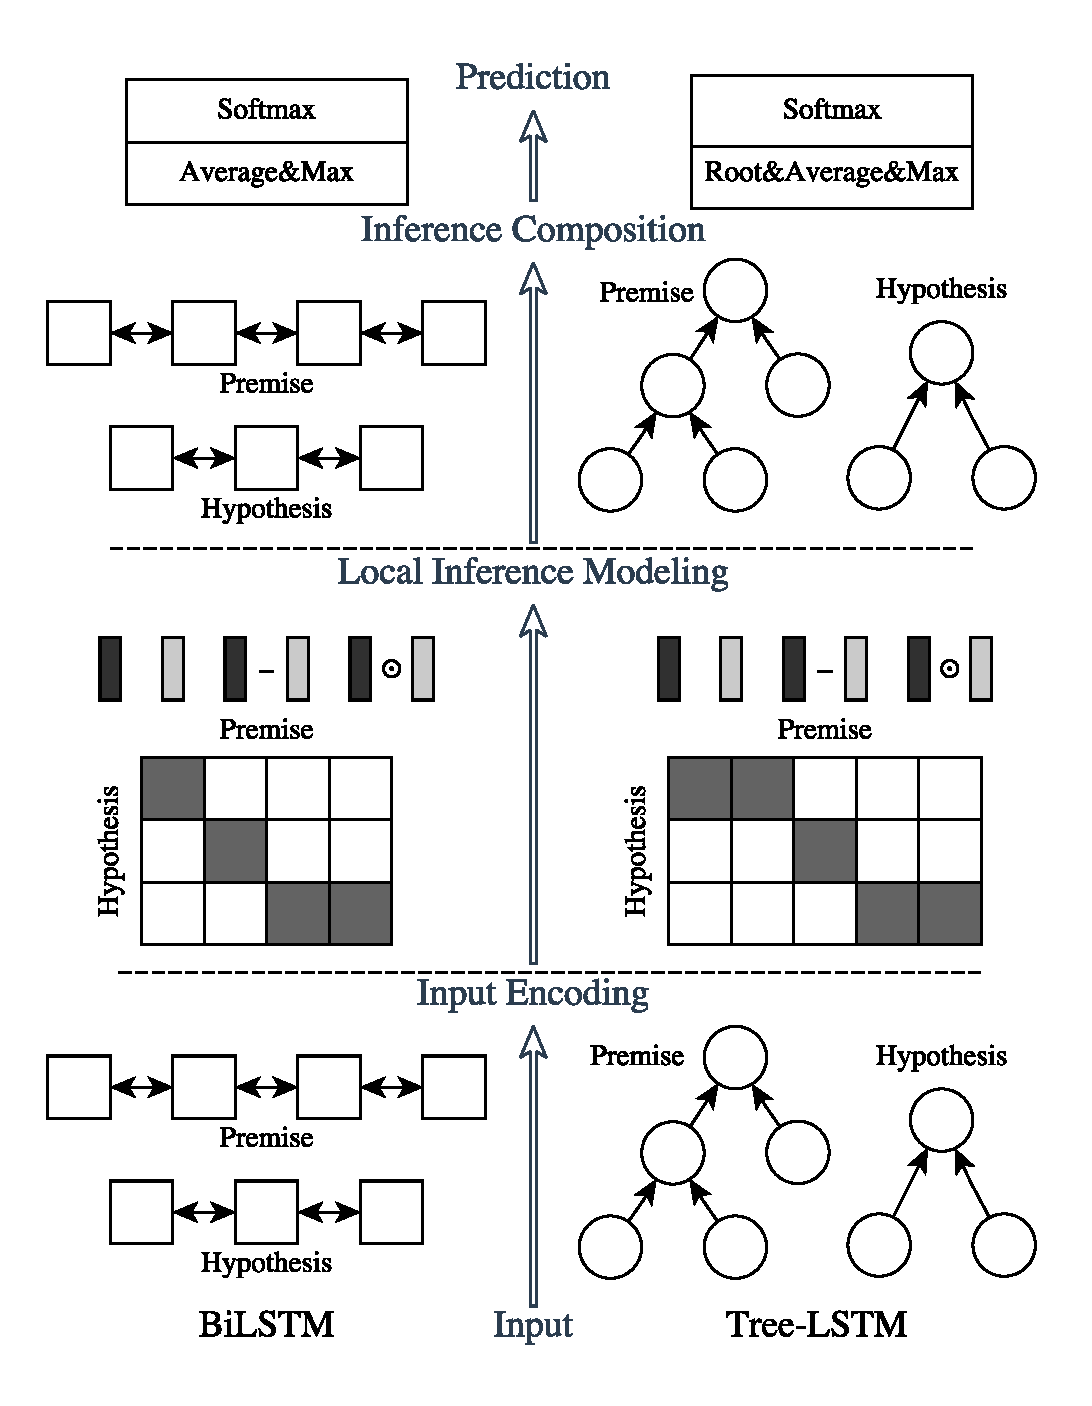
\includegraphics[scale=0.3]{esim.eps}
	
	\end{figure}
\footnotetext{\citep{esim16}}
}


\frame[<+->]{
	\frametitle{Machine translation}

\begin{figure}
   \includegraphics[width=0.25\textwidth]{mtgoog}
   \hfill
   \includegraphics[width=0.75\textwidth]{nmt_eg}
\end{figure}	
	

	
\footnotetext{\citep{BahdanauCB14}}
}

\frame[<+->]{
	\frametitle{Machine translation}

	 \animategraphics[loop,controls,width=\linewidth]{10}{seq2seq_gif/seq2seq-}{0}{214}

}


\frame[<+->]{
	\frametitle{Question answering}

	\begin{figure}
	\includegraphics[scale=0.2]{QA}
	
	\end{figure}
\footnotetext{\citep{smerity}}

}

\frame[<+->]{
	\frametitle{Question answering}

	
	\begin{figure}
	\includegraphics[scale=0.35]{qa_nn1}
	
	\end{figure}

}


\frame[<+->]{
	\frametitle{Sentiment classification}
\begin{figure}
   \includegraphics[width=0.55\textwidth]{sentiment}
   \hfill
   \includegraphics[width=0.35\textwidth]{sentiment2}
\end{figure}

\footnotetext{\url{https://www.edgarsdatalab.com/2017/09/04/sentiment-analysis-using-tidytext/}}
}


\frame[<+->]{
	\frametitle{Sentiment classification}

	\begin{figure}
	\includegraphics[scale=0.45]{treeLSTM}
	
	\end{figure}
\footnotetext{\citep{treelstm}}
}


\frame[<+->]{
	\frametitle{Graphical Models}
	\centering{
	\begin{tikzpicture}
    % Define nodes
    \node[obs]		(x)		{$ x $};
    \node[obs, below = of x]		(y)		{$ y $};
    \node[right = of y]		(theta)		{$ \theta $};
    
    
    % Connect nodes
    \edge{x,theta}{y};
    
    % add plates
    \plate {x-sentence} {(y)(x)} {$ m $};
    \end{tikzpicture}	
	}

}




\frame[<+->]{
	\frametitle{Supervised learning}
	\begin{itemize}
	\item We have data inputs $X = \langle x_1, \ldots, x_n  \rangle$, and the corresponding outputs $Y = \langle y_1, \ldots, y_n \rangle$ \\
	generated by some unknown procedure
	\item which we assume can be captured by a probabilistic model \\
	 with known probability (mass/density) function e.g.
		\begin{equation}
		\begin{aligned}
    			p(y|x, \theta ) = \Cat(y|f(x; \theta)) ,
		\end{aligned}
		\end{equation}

	\item $y$ outputs computed by mapping from the input to the class probabilities with a neural network $f$ parameterised by $\theta$ 
	\item \cblue{Goal} estimate parameters that assign maximum likelihood to observations
	\end{itemize}
	

}

\frame[<+->]{
	\frametitle{Supervised learning}
	\begin{tabular}{ccc}
                    & x                   & y                   \\
	Parsing             & Sentence            & Syntactic tree      \\
	Machine translation & Source              & Target translation  \\
	NLI                 & Text and Hypohtesis & Entailment relation
	\end{tabular}
	

}



\frame[<+->]{
	\frametitle{Supervised learning}

	
	\begin{figure}
	\includegraphics[scale=0.2]{supervised1}
	
	\end{figure}
\footnotetext{\citep{neubigtalk}}
}

\frame[<+->]{
	\frametitle{Supervised learning}

	\begin{figure}
	\includegraphics[scale=0.2]{supervised2}
	
	\end{figure}
\footnotetext{\citep{neubigtalk}}
}

\frame[<+->]{
	\frametitle{Supervised learning}

	
	\begin{figure}
	\includegraphics[scale=0.2]{supervised3}
	
	\end{figure}
\footnotetext{\citep{neubigtalk}}
}

\frame[<+->]{
	\frametitle{Supervised learning}

	
	\begin{figure}
	\includegraphics[scale=0.2]{supervised4}
	
	\end{figure}
\footnotetext{\citep{neubigtalk}}
}

\frame[<+->]{
	\frametitle{Supervised learning}
	\begin{itemize}
	\item Maximum likelihood estimation tells you which loss to optimise
(i.e. negative log-likelihood)
	\item Automatic differentiation (backprop) chain rule of derivatives:\\ 
	give a tractable forward pass and get gradients
	\item Stochastic optimisation powered by backprop
general purpose gradient-based optimisers
	\end{itemize}
	
}

\frame[<+->]{
	\frametitle{Maximum likelihood estimation}
	\begin{itemize}
	\item Let $p(y \mid \theta)$ be the probability of an observation $y$ and $\theta$ refer to all of its parameters \\
	Given a dataset $y^{(1)},...,y^{(N)}$ of i.i.d. observations,\\
	 the log-likelihood function gives us a criterion for parameter estimation

	\begin{equation}
	\begin{aligned}
	\Lagr(\theta \mid  y^{(1:N)})  = log \prod_{s=1}^{N}p(y^{(N)} \mid  \theta) = \sum_{s=1}^{N} log p(y^{(N)} \mid  \theta) 
	\end{aligned}
	\end{equation}

	\end{itemize}
	
}


\frame[<+->]{
	\frametitle{MLE via gradient-based optimisation}
	\begin{itemize}
	\item If the log-likelihood is \cblue{differentiable} and \cblue{tractable} then backprop gives us the gradient

	\begin{equation}
	\begin{aligned}
	\nabla_{\theta} \Lagr(\theta \mid y^{(1:N)} ) &= \nabla_{\theta} \sum_{s=1}^{N}log p(y^{(N)} \mid  \theta) \\
	&= \sum_{s=1}^{N}\nabla_{\theta} log p(y^{(N)} \mid  \theta)
	\end{aligned}
	\end{equation}
	\item and we can update $\theta$ in the direction
	\begin{equation}
	\begin{aligned}
	\gamma \nabla_{\theta} \Lagr(\theta \mid y^{(1:N)})
	\end{aligned}
	\end{equation}
	
	to achieve  a local maximum of the likelihood function
	\end{itemize}
	
}




\frame[<+->]{
	\frametitle{Latent variable approach}
\begin{itemize}
\item Because NN models work but they may struggle with:
\item lack of training data
\item partial supervision
\item lack of inductive bias
\end{itemize}
	

}


\frame[<+->]{
	\frametitle{Latent variable approach}

	\begin{figure}
	\includegraphics[scale=0.2]{unsupervised}
	
	\end{figure}
\footnotetext{\citep{neubigtalk}}
	

}

\frame[<+->]{
	\frametitle{Latent variable approach}

	\begin{figure}
	\includegraphics[scale=0.43]{unsupervised2}
	
	\end{figure}
\footnotetext{\citep{neubigtalk}}
	

}





\section{Course Topics}


\frame[<+->]{
	\frametitle{What is this course?}
	\begin{figure}
	\includegraphics[scale=0.43]{ibm_lectures}
	
	\end{figure}

}

\frame[<+->]{
	\frametitle{What is this course?}
	\begin{figure}
	\includegraphics[scale=0.43]{word_alignment}
	
	\end{figure}

}

\frame[<+->]{
	\frametitle{What is this course?}
	\begin{figure}
	\includegraphics[scale=0.43]{ibm_lectures}
	
	\end{figure}

}


\frame[<+->]{
	\frametitle{What is this course?}
	\begin{figure}
	\includegraphics[scale=0.4]{vae_lectures2}
	\end{figure}

}

\frame[<+->]{
	\frametitle{What is this course?}
	\begin{figure}
	\includegraphics[scale=0.4]{vae_lectures1}
	\end{figure}

}

\frame[<+->]{
	\frametitle{Goals}
	\begin{itemize}
	\item Go through current literature
	\item Define probabilistic models
	\item Start combining probabilistic models and NN architectures
	
	\end{itemize}
	

}

\frame[<+->]{
	\frametitle{Next class}
	\begin{itemize}
	\item Probabilistic Graphical Models 
	\item Introduction to Word Alignment
	\end{itemize}

}






